\documentclass[18pt]{beamer}
\usepackage[utf8]{inputenc} % for the umlauts
\usepackage{subfigure}

\beamertemplatenavigationsymbolsempty
%% SLIDE FORMAT

% use 'beamerthemekit' for standard 4:3 ratio
% for widescreen slides (16:9), use 'beamerthemekitwide'

\usepackage{templates/beamerthemekit}
% \usepackage{templates/beamerthemekitwide}

\setcounter{tocdepth}{1}

%% TITLE PICTURE

% if a custom picture is to be used on the title page, copy it into the 'logos'
% directory, in the line below, replace 'mypicture' with the 
% filename (without extension) and uncomment the following line
% (picture proportions: 63 : 20 for standard, 169 : 40 for wide
% *.eps format if you use latex+dvips+ps2pdf, 
% *.jpg/*.png/*.pdf if you use pdflatex)

%\titleimage{mypicture}

%% TikZ INTEGRATION

% use these packages for PCM symbols and UML classes
% \usepackage{templates/tikzkit}
% \usepackage{templates/tikzuml}

% the presentation starts here

\usepackage{mathabx}
\usepackage{picture}
\usepackage[absolute,overlay]{textpos}
%\usepackage[texcoord,grid,gridunit=mm,gridcolor=red, subgridcolor=green]{eso-pic}
\setbeamercovered{invisible}
\setbeamertemplate{caption}{\raggedright\insertcaption\par}

\title[SWT1]{Softwaretechnik 1 - 5. Tutorium}
\subtitle{Tutorium 03}
\author{Felix Bachmann}
\date{10.07.2017}

\institute{KIT - Institut für Programmstrukturen und Datenorganisation (IPD)}

% Bibliography

\usepackage[citestyle=authoryear,bibstyle=numeric,hyperref,backend=biber]{biblatex}
\addbibresource{templates/example.bib}
\bibhang1em

\begin{document}
	
% change the following line to "ngerman" for German style date and logos
\selectlanguage{ngerman}
	
%title page
\begin{frame}
\titlepage
\end{frame}

\begin{frame}
\tableofcontents
\end{frame}


\section{Orga}

	\subsection{Allgemein}
	\begin{frame}
		\frametitle{Allgemeines}
		\begin{alertblock}{Nächstes Mal letztes Tutorium} 
		\begin{itemize}
			\item irgendwelche Wünsche für das letzte Tut?
			\begin{itemize}
				\item etwas bestimmtes wiederholen?
				\item falls euch noch was einfällt, schreibt mir eine Mail
				\linebreak $\implies$ felix.bachmann@ewetel.net
			\end{itemize}
		\end{itemize}
		\end{alertblock}
		\pause
		\begin{block}{Evaluation vom letzten Mal}
			\begin{itemize}
				\item nochmal Danke fürs Mitmachen! \pause
				\item häufigster Kritikpunkt: nicht so gut lesbarer Tafelanschrieb
				\linebreak $\implies$ versuche ich besser zu machen :)
			\end{itemize}
		\end{block}
	\end{frame}

	\subsection{Feedback 4. Übungsblatt}
	\begin{frame}
		\frametitle{4. Übungsblatt Statistik}
		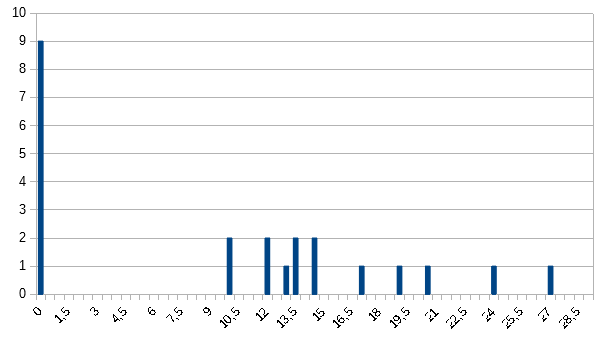
\includegraphics[scale=0.7]{./pics/tut5/statistics-ub5.png}
		\linebreak \centering $\diameter$ 13 bzw 18,4 von 25+8
	\end{frame}

	\begin{frame}
		\frametitle{4. Übungsblatt - Häufige Fehler (A3)}
		\begin{block}{Aufgabe 3 (GUI für Geometrify): 6,56 bzw. 11,25 von 10+7} 
			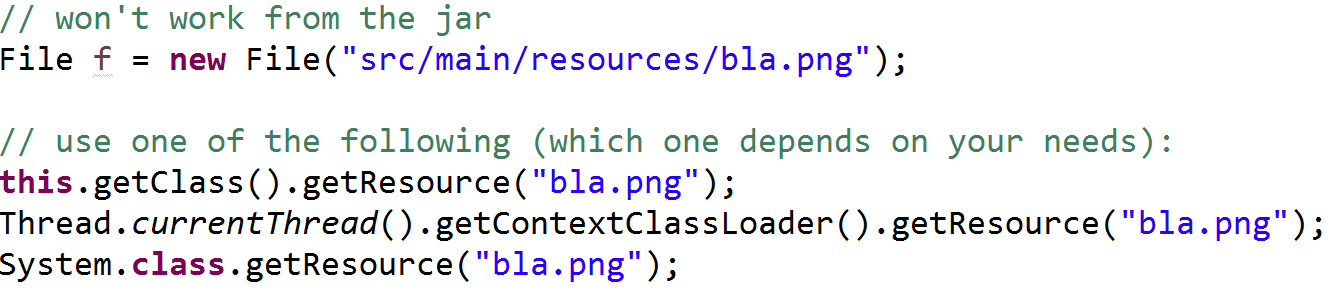
\includegraphics[scale=0.34]{./pics/tut5/file-resource.png}
			\begin{itemize}
				\pause
				\item keine leeren JPanels o.a. Objekte benutzen, um Platz zwischen Objekten zu erzeugen
				\linebreak $\implies$ geht schöner, performanter mit LayoutManagern \pause
				\item fileChooser.setFileFilter(filter) anstatt fileChooser.addChoosableFileFilter(filter)
			\end{itemize}
			mehr zur Aufgabe 3 nach dem Parallelität-Teil!
		\end{block}
	\end{frame}


	\subsection{Feedback 5. Übungsblatt}
	\begin{frame}
		\frametitle{5. Übungsblatt Statistik}
		%TODO statistics 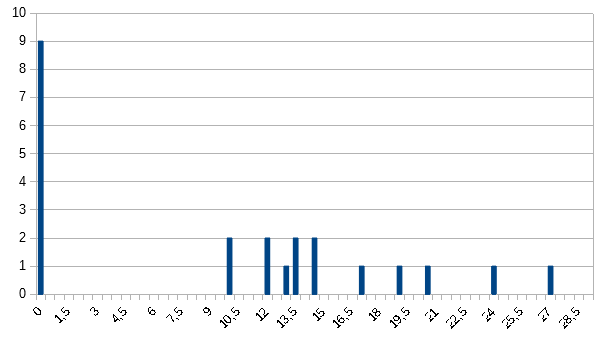
\includegraphics[scale=0.7]{./pics/tut5/statistics-ub5.png}
		%\linebreak \centering $\diameter$ %TODO avg
	\end{frame}

	\subsection{5. Übungsblatt - Fehler (Allgemein)}
	\begin{frame}
		\frametitle{Häufige Fehler}
		\begin{block}{Allgemein}
			\begin{itemize}
				\item %TODO common faults
			\end{itemize}
		\end{block}
	\end{frame}

	\subsection{5. Übungsblatt - Fehler}
	\begin{frame}
		\frametitle{Häufige Fehler}
		\begin{block}{Aufgabe 1 (Architekturstile): $\diameter$   von 5} %TODO avg
			\begin{itemize}
				\pause 
				\item %TODO 
			\end{itemize}
		\end{block}
	\end{frame}

	\begin{frame}
		\frametitle{Häufige Fehler}
		\begin{block}{Aufgabe 2 (Iterator für Plug-Ins): $\diameter$ von 6} %TODO avg
			\begin{itemize}
				\pause 
				\item %TODO
			\end{itemize}
		\end{block}
		\pause 
		\begin{block}{Aufgabe 3 (Umstrukturierung von Geometrify): $\diameter$ von 8} %TODO avg
			\begin{itemize}
				\item %TODO
			\end{itemize}
		\end{block}
	\end{frame}

	\begin{frame}
		\frametitle{Häufige Fehler}
		\begin{block}{Aufgabe 4 (Reimplementierung von Geometrify): $\diameter$ von 7+2} %TODO avg
			\begin{itemize}
				\pause
				\item %TODO
			\end{itemize}
		\end{block}
	\end{frame}

\section{Recap}
	\subsection{Kontext}
	
	
	
\section{Parallelität}
	\subsection{}	
	
	%TODO parallelism
	
	
	\begin{frame}
		\frametitle{4. Übungsblatt - A3 mit Threads}
		\begin{block}{Aufgabe 3 (GUI für Geometrify): 6,56 bzw. 11,25 von 10+7} 
			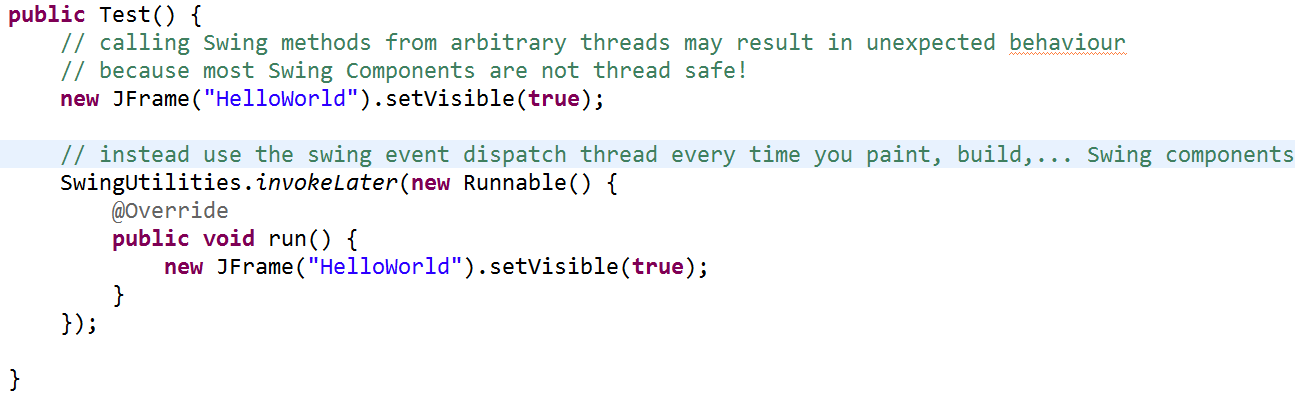
\includegraphics[scale=0.34]{./pics/tut5/edt.png}
		\end{block}
	\end{frame}

	\begin{frame}
		\frametitle{4. Übungsblatt - A3 mit Threads}
		\begin{block}{Aufgabe 3 (GUI für Geometrify): 6,56 bzw. 11,25 von 10+7} 
			\centering
			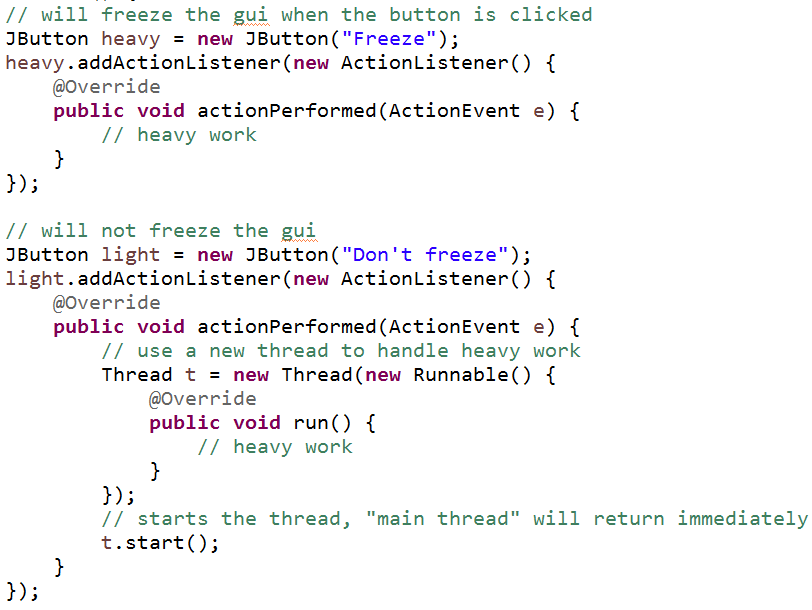
\includegraphics[scale=0.34]{./pics/tut5/extra-thread.png}
		\end{block}
	\end{frame}

\section{Testen}
	\subsection{}


\section{Tipps}
	\subsection{Tipps}
	\begin{frame}
		\frametitle{Tipps - 6. Übungsblatt}
		\begin{exampleblock}{Aufgabe 1: Kontrollfluss-orientiertes Testen}
			\begin{itemize}
				\item Zwischensprache benutzen
				\item Definitionen der verschiedenen Abdeckungen anschauen
			\end{itemize}
		\end{exampleblock}
		\pause
		\begin{exampleblock}{Aufgabe 2: Codeinspektion} 
			\begin{itemize}
				\item an das Format halten
			\end{itemize}
		\end{exampleblock}
	\end{frame}

	\begin{frame}
		\frametitle{Tipps - 6. Übungsblatt}
		\begin{exampleblock}{Aufgabe 3: Parallelisierung von Geometrify}
			\begin{itemize}
				\item Berechnung der Samples parallelisieren
				\item Zahl der benutzten Threads abhängig machen von der Anzahl der Prozessor-Kerne
			\end{itemize}
		\end{exampleblock}
		\pause
		\begin{exampleblock}{Aufgabe 4: Alternative Parallelisierungsverfahren}
			\begin{itemize}
				\item theoretische Überlegungen, was man sonst noch so parallelisieren könnte
				\item Sinnhaftigkeit, Aufwand, etc. prüfen
			\end{itemize}
		\end{exampleblock}
	\end{frame}

	\begin{frame}
		\frametitle{Tipps - 6. Übungsblatt}
		\begin{exampleblock}{Aufgabe 5: Parallelisierungswettbewerb}
			\begin{itemize}
				\item Aufgabe 3 verbessern und Laufzeit messen
			\end{itemize}
		\end{exampleblock}
	\end{frame}

	\subsection{Abgabe}
	\begin{frame}
		\frametitle{Denkt dran!}
		\begin{alertblock}{Abgabe}
			\begin{itemize}
				\item Deadline am 19.7. um 12:00
				\item Aufgabe 1,2,4 und Beschreibung, Laufzeitprofil von Aufgabe 5 handschriftlich
			\end{itemize}
		\end{alertblock}
	\end{frame}

	\begin{frame}
		\frametitle{Bis dann! (dann  := 24.07.17)}
		\centering
		
\includegraphics[scale=1.0]{./comics/geek_and_poke_concurrency.jpg}
	\end{frame}

\end{document}